\subsection{Introduction}

\begin{frame}[containsverbatim]
	\frametitle{What will we learn today ?}	
	\begin{itemize}
		\item {Hybrid programming models comparison
			\begin{itemize}
				\item {Pure MPI}
				\item {MPI+OpenMP}
				\item {(MPI + MPI one-sided (MPI-3) )}
			\end{itemize}
		}
		\item {How to write a (production) project proposal}
	\end{itemize}
\end{frame}


\subsection{Hybrid programming models}


\begin{frame}[containsverbatim]
	\frametitle{Situation}	

\hspace*{2mm}% Slide 258
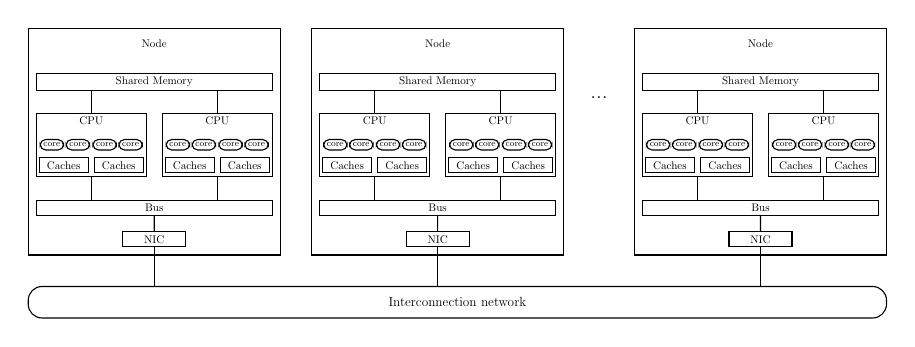
\begin{tikzpicture}[scale=0.4, every node/.style={scale=0.4}]

\pgfmathsetmacro{\lastxstart}{19}

\foreach \x[count = \i] in {-0.25, 8.75, \lastxstart} {
	\begin{scope}[xshift = \x cm]
	\draw (0.25,0) rectangle (8.25, 7.2);

	\node[draw, rectangle, minimum width = 2cm] (NIC\i) at (4.25, 0.5) {NIC};
	\node[draw, rectangle, minimum width = 7.5cm] (Bus) at (4.25, 1.5) {Bus};
	\node[draw, rectangle, minimum width = 7.5cm] (Shared) at (4.25, 5.5) {Shared Memory};
	\node at (4.25, 6.7) {Node};

	\begin{scope}[xshift = 2.25cm, yshift = -0.5cm]
	\node[rectangle, draw, minimum height = 2cm, minimum width = 3.5cm] (CPU1) at (0, 4) {};
	\node[below] at (CPU1.north) {CPU};

	\foreach \x in {-1.25, -0.425, 0.425, 1.25}
		\node[draw, rectangle, rounded corners = 2pt, inner sep = 3pt] at (\x, 4) {\footnotesize core};

	\foreach \x in {0.875, -0.875}
		\node[draw, rectangle, minimum width = 1.55cm] at (\x, 3.35) {Caches};
	\end{scope}

	\begin{scope}[xshift = 6.25cm, yshift = -0.5cm]
	\node[rectangle, draw, minimum height = 2cm, minimum width = 3.5cm] (CPU2) at (0, 4) {};
	\node[below] at (CPU2.north) {CPU};

	\foreach \x in {-1.25, -0.425, 0.425, 1.25}
		\node[draw, rectangle, rounded corners = 2pt, inner sep = 3pt] at (\x, 4) {\footnotesize core};

	\foreach \x in {0.875, -0.875}
		\node[draw, rectangle, minimum width = 1.55cm] at (\x, 3.35) {Caches};
	\end{scope}

	\draw (CPU1 |- Shared.south) -| (CPU1.north);
	\draw (CPU2 |- Shared.south) -| (CPU2.north);

	\draw (CPU1 |- Bus.north) -| (CPU1.south);
	\draw (CPU2 |- Bus.north) -| (CPU2.south);

	\draw (Bus) -- (NIC\i);
	\end{scope}
}

\pgfmathsetmacro{\lastx}{\lastxstart + 8.25}

\node[draw, rectangle, rounded corners = 5pt, minimum width = \lastx cm, minimum height = 1cm] (ICN) at ({\lastx / 2}, -1.5) {\large Interconnection network};

\draw (NIC1 |- ICN.north) -| (NIC1.south);
\draw (NIC2 |- ICN.north) -| (NIC2.south);
\draw (NIC3 |- ICN.north) -| (NIC3.south);

\node at (18.125, 5) {\huge ...};

\end{tikzpicture}


\end{frame}



\begin{frame}[containsverbatim]
	\frametitle{Situation}	

\vspace*{2mm}% Slide 259
\begin{tikzpicture}[scale=0.4, every node/.style={scale=0.4}]

\pgfmathsetmacro{\lastxstart}{19}

\foreach \x[count = \i] in {-0.25, 8.75, \lastxstart} {
	\begin{scope}[xshift = \x cm]
	\draw (0.25,0) rectangle (8.25, 7.2);

	\node[draw, rectangle, minimum width = 2cm] (NIC\i) at (4.25, 0.5) {NIC};
	\node[draw, rectangle, minimum width = 7.5cm] (Bus) at (4.25, 1.5) {Bus};
	\node[draw, rectangle, minimum width = 7.5cm] (Shared) at (4.25, 5.5) {Shared Memory};
	\node at (4.25, 6.7) {Node};

	\begin{scope}[xshift = 2.25cm, yshift = -0.5cm]
	\node[rectangle, draw, minimum height = 2cm, minimum width = 3.5cm] (CPU1) at (0, 4) {};
	\node[below] at (CPU1.north) {CPU};

	\foreach \x in {-1.25, -0.425, 0.425, 1.25}
		\node[draw, rectangle, rounded corners = 2pt, inner sep = 3pt] at (\x, 4) {\footnotesize core};

	\foreach \x in {0.875, -0.875}
		\node[draw, rectangle, minimum width = 1.55cm] at (\x, 3.35) {Caches};
	\end{scope}

	\begin{scope}[xshift = 6.25cm, yshift = -0.5cm]
	\node[rectangle, draw, minimum height = 2cm, minimum width = 3.5cm] (CPU2) at (0, 4) {};
	\node[below] at (CPU2.north) {CPU};

	\foreach \x in {-1.25, -0.425, 0.425, 1.25}
		\node[draw, rectangle, rounded corners = 2pt, inner sep = 3pt] at (\x, 4) {\footnotesize core};

	\foreach \x in {0.875, -0.875}
		\node[draw, rectangle, minimum width = 1.55cm] at (\x, 3.35) {Caches};
	\end{scope}

	\draw (CPU1 |- Shared.south) -| (CPU1.north);
	\draw (CPU2 |- Shared.south) -| (CPU2.north);

	\draw (CPU1 |- Bus.north) -| (CPU1.south);
	\draw (CPU2 |- Bus.north) -| (CPU2.south);

	\draw (Bus) -- (NIC\i);

	\draw[blue2, thick, rounded corners = 5pt] (0.375, 0.95) rectangle (8.125, 6.2);
	\node[above, blue2] at (7, 6.2) {OpenMP};

	\end{scope}
}

\pgfmathsetmacro{\lastx}{\lastxstart + 8.25}

\node[draw, rectangle, rounded corners = 5pt, minimum width = \lastx cm, minimum height = 1cm] (ICN) at ({\lastx / 2}, -1.5) {\large Interconnection network};

\draw (NIC1 |- ICN.north) -| (NIC1.south);
\draw (NIC2 |- ICN.north) -| (NIC2.south);
\draw (NIC3 |- ICN.north) -| (NIC3.south);

\node at (18.125, 5) {\huge ...};


\draw[thick, yellowbrown2, rounded corners = 5pt] (-0.5, -2.2) rectangle (\lastx + 0.5, 0.85);
\node[below, yellowbrown2] at (18, -2.2) {\Large MPI between nodes};

\end{tikzpicture}


\end{frame}

\begin{frame}[containsverbatim]
	\frametitle{Situation : problems}	
\begin{itemize}
	\item {Thread safety ?}
	\item {Which thread/process can/will call the MPI library ?}
	\item {MPI process placement in the case of multi-CPU processors ?}
	\item {Data visibility ? OpenMP private ? }
	\item {Does my problem fits with the targeted machine ?}
	\item {Levels of parallelism within my problem ?}
\end{itemize}
\end{frame}



\begin{frame}[containsverbatim]
	\frametitle{Hybrid vs. Pure MPI}	
\textbf{Pure MPI}
\begin{itemize}
	\item {\textbf{+} no code modification}
	\item {\textbf{+} most of the libraries support multi-thread}
	\item {\textbf{-} does application topology fits system topology ?}
	\item {\textbf{-} useless communications}
\end{itemize}
\textbf{Hybrid}
\begin{itemize}
	\item {\textbf{+} no message within an SMP node}
	\item {\textbf{+} less (no) topology problems}
	\item {\textbf{-} all threads sleep when master communicates}
	\item {\textbf{-} MPI-libs must support (at least) thread safety}
\end{itemize}
\end{frame}


\begin{frame}[containsverbatim]
\frametitle{Hybrid MPI/OpenMP hello world}
\begin{lstlisting}[language=C,frame=lines]
int main(int argc, char *argv[]) {
  int numprocs, rank, namelen,provided;
  char processor_name[MPI_MAX_PROCESSOR_NAME];
  int iam = 0, np = 1;
  MPI_Init_thread(&argc, &argv,MPI_THREAD_SINGLE,provided);
  MPI_Comm_size(MPI_COMM_WORLD, &numprocs);
  MPI_Comm_rank(MPI_COMM_WORLD, &rank);
  #pragma omp parallel default(shared) private(iam, np)
  {
    np = omp_get_num_threads();
    iam = omp_get_thread_num();
    printf("Hello from thread %d out of %d from process %d out of %d on\n",iam, np, rank, numprocs);
  }
  MPI_Finalize();
}
\end{lstlisting}

Need to overlap communications (from master) with computation between the others. If possible !

\end{frame}



\begin{frame}[containsverbatim]
\frametitle{Hybrid MPI/OpenMP hello world}

  Compilation using the GNU gcc compiler:
\begin{verbatim}
mpicc -fopenmp hello.c -o hello
\end{verbatim}
  Compilation using the Intel C compiler:

\begin{verbatim}
mpiicc -qopenmp hello.c -o hello
\end{verbatim}

Warning : when using Intel MPI : it is mandatory to link against the thread-safe library (-mt$\_$mpi) or at least to check if the executable has been linked against this lib (\verb+ldd hello+ should print \verb+libmpi_mt.so.XX+) if \verb+mpiicc+ or \verb+mpiifort+ has been used.

\end{frame}


\begin{frame}[containsverbatim]
\frametitle{Submission script the clusters}

\begin{verbatim}
#!/bin/bash
#SBATCH --nodes 2
#SBATCH --ntasks 2
#SBATCH --cpus-per-task 16
#SBATCH --ntasks-per-node=1
#SBATCH --time 00:00:30
#SBATCH --workdir /scratch/vkeller

module purge
module load intel intel-mpi

export OMP_NUM_THREADS=$SLURM_CPUS_PER_TASK
srun ./hello 
\end{verbatim}

It will start 2 MPI processes each will spawn 16 threads

\end{frame}













\begin{frame}[fragile]
\frametitle{Changes to your code}
\begin{itemize}
\item change your MPI initialisation routine
\begin{itemize}
    \item \verb+MPI_Init+ is replaced by \verb+MPI_Init_thread+
    \item \verb+MPI_Init_thread+ has two additional parameters for the level of thread support
        required, and for the level of thread support provided by the library implementation
\end{itemize}

\begin{Verbatim}[formatcom=\color{blue}]
int MPI_Init_thread(int *argc, char ***argv, 
                      int required, int *provided)
\end{Verbatim}

       \textcolor{dkgreen}{required specifies       the     requested       level   of      thread  support,        and     the     actual  level   of      support is      then    returned        into    provided}

\item add OpenMP directives or Pthread calls as long as you stick to the level of thread safety you specified in the call to \verb+MPI_Init_thread+
\end{itemize}

\end{frame}


\begin{frame}[fragile]
\frametitle{The 4 Options for Thread Support}
%\framesubtitle{I: user informs the MPI library}


\begin{itemize}
\item \verb+MPI_THREAD_SINGLE+
\begin{itemize}
\item Only one thread will execute
\item Standard MPI-only application
\end{itemize}
\item \verb+MPI_THREAD_FUNNELED+
\begin{itemize}
\item Only the Master Thread will make calls to the MPI library
%\item $\rightarrow$ The thread that calls \verb+MPI_Init_thread+ is the master thread
\item A thread can determine whether it is the master thread by a call to \verb+MPI_Is_thread_main+
\end{itemize}
\item \verb+MPI_THREAD_SERIALIZED+
\begin{itemize}
\item Only one thread at a time will make calls to the MPI library, but all threads are eligible to make such calls
\end{itemize}
\end{itemize}

%\begin{Verbatim}[formatcom=\color{blue}]
%int MPI_Is_main_thread(int * flag);
%\end{Verbatim}
\end{frame}


\begin{frame}[fragile]
\frametitle{The 4 Options for Thread Support}
%\framesubtitle{II: The MPI Library is responsible for Thread Safety}

\begin{itemize}
\item \verb+MPI_THREAD_MULTIPLE+
\begin{itemize}
\item Any thread may call the MPI library at any time
\item The MPI library is responsible  for thread safety within that library, and for any libraries that  it in turn uses
\item Codes that rely on the level of \verb+MPI_THREAD_MULTIPLE+ may run significantly slower than the  case where one of the other options has been chosen
\item You might need to link in a separate library in order to get this level of support
\end{itemize}
\end{itemize}


    In  most    cases   \verb+MPI_THREAD_FUNNELED+      provides        the     best    choice  for     hybrid  programs

\begin{Verbatim}[formatcom=\color{blue}]
int MPI_Query_thread( int * thread_level_provided);
\end{Verbatim}

Returns the level of thread support provided by the MPI library

\end{frame}



\begin{frame}
\frametitle{Topology problems}

%The problem: we have a domain with 80 subdomains as follows:
%
%\begin{center}
%\begin{tikzpicture}%
%  \draw[step=4mm] (0,0) grid (6.4,2.0);
%\end{tikzpicture}
%\end{center}

How to deal with :

\begin{itemize}
\item topology / mapping ? (Which physical core is assigned to which process/thread)
\item sub-domain decomposition ?
\item halos size ? halos shapes ?
\item unnecessary communications ?
\item \textbf{computation to communication ratio} ?
\end{itemize}

Pure MPI ? Hybrid ?
\\
\textbf{A good solution is : one MPI process per ``SMP'' node}

\end{frame}



\begin{frame}
\frametitle{Halo regions}
% Neil, p. 54
\begin{itemize}
\item  Halo regions are local copies of remote data that are needed for computations
\item  Halo regions need to be copied fequently
\item  Using threads reduces the size of halo region copies that need to be stored
\item  Reducing halo region sizes also reduces communication requirements
\end{itemize}
\end{frame}



\begin{frame}
\frametitle{Take-home messages}
\begin{itemize}
\item Always take into account the problems related to the physical topology
\item A real application is not as easy as a hello world.
\item Some clusters have different connectivity topologies: match them to your problem. Examples of hardware topologies :
\begin{itemize}
\item all-to-all
\item 2D/3D torus
\item tree
\item ...
\end{itemize}
        \item One MPI process per physical node 
\end{itemize}
\end{frame}





\begin{frame}[fragile]
\frametitle{Main messages}
\begin{itemize}
\item Do not use hybrid if the pure MPI code scales ok
\item Be aware of intranode MPI behavior
\item Always observe the topology dependence of
\begin{itemize}
   \item Intranode MPI
   \item Threads overheads
\end{itemize}
\item Finally: Always compare the best pure MPI code with the best hybrid code!
\end{itemize}

\end{frame}


\begin{frame}[fragile]
\frametitle{Examples that \textit{can} benefit of an hybrid approach}
\begin{itemize}
\item MPI codes with a lot of all-to-all communications
\item MPI codes with a very poor load balancing at the algorithmic level (less communications)
\item MPI codes with memory limitations
\item MPI codes that can be easily \textit{fine-grained parallelized} (at loop level)
\item MPI codes that will offload codes on accelerators
\end{itemize}

\end{frame}





%%% Local Variables: 
%%% mode: latex
%%% TeX-master: "../cours_vince"
%%% End: 
